% Methods note. Build: pdflatex note.tex three times (see ../README.md). Every number in the text comes from
% numbers.tex and the tab_*.tex fragments, which ../code/make_numbers.py writes from the outputs in ../out/;
% the figures are written by ../code/make_figures.py.
\documentclass[11pt]{article}
\usepackage[letterpaper,margin=1in]{geometry}
\usepackage[T1]{fontenc}
\usepackage{lmodern}
\usepackage{amsmath,amssymb,amsthm}
\usepackage{graphicx}
\usepackage{array}
\usepackage{booktabs}
\usepackage{microtype}
\usepackage[font=small,skip=4pt]{caption}
\usepackage[hidelinks]{hyperref}

\hypersetup{
  pdftitle={A finite rank window cannot show that a neural population code satisfies the eigenspectrum smoothness bound},
  pdfauthor={Chase Hendrick}}

\newtheorem{proposition}{Proposition}
\newtheorem{corollary}{Corollary}
\theoremstyle{definition}
\newtheorem{remark}{Remark}

\renewcommand{\topfraction}{0.9}
\renewcommand{\textfraction}{0.1}
\renewcommand{\floatpagefraction}{0.8}

% Generated by code/make_numbers.py from ../out/. Do not edit.
\newcommand{\ChiFourMed}{3.36}
\newcommand{\ChiFourQ}{9.49}
\newcommand{\CrossAboveEight}{1}
\newcommand{\CrossAboveFour}{1}
\newcommand{\CrossBelowEight}{1/4}
\newcommand{\CrossBelowFour}{1/2}
\newcommand{\CurvBorderReachMax}{0.33}
\newcommand{\CurvBorderReachMin}{0.24}
\newcommand{\CurvBorderReachN}{7}
\newcommand{\CurvMax}{$+0.83$}
\newcommand{\CurvMedEight}{0.21}
\newcommand{\CurvMin}{$-0.76$}
\newcommand{\DeffEightMax}{4.4}
\newcommand{\DeffEightMin}{3.2}
\newcommand{\DeffFourMax}{2.7}
\newcommand{\DeffFourMin}{2.6}
\newcommand{\DeffMidEightMax}{5.1}
\newcommand{\DeffMidEightMin}{3.5}
\newcommand{\DeffMidFourMax}{2.9}
\newcommand{\DeffMidFourMin}{2.8}
\newcommand{\DnnEightMax}{7.0}
\newcommand{\DnnEightMin}{5.2}
\newcommand{\DnnFourMax}{3.0}
\newcommand{\DnnFourMin}{2.8}
\newcommand{\DnnGaussEightMax}{7.9}
\newcommand{\DnnGaussEightMin}{6.1}
\newcommand{\DnnGaussFourMax}{4.3}
\newcommand{\DnnGaussFourMin}{3.8}
\newcommand{\DnnGaussIsoEightMax}{8.1}
\newcommand{\DnnGaussIsoEightMin}{7.2}
\newcommand{\DnnGaussIsoFourMax}{4.2}
\newcommand{\DnnGaussIsoFourMin}{3.9}
\newcommand{\DnnWhiteEightMax}{7.4}
\newcommand{\DnnWhiteEightMin}{6.5}
\newcommand{\DnnWhiteFourMax}{3.0}
\newcommand{\DnnWhiteFourMin}{2.9}
\newcommand{\FinBorderShiftMax}{$-0.002$}
\newcommand{\FinBorderShiftMin}{$-0.046$}
\newcommand{\FinCells}{112}
\newcommand{\FinCrossAboveEight}{2}
\newcommand{\FinCrossAboveFour}{1}
\newcommand{\FinCrossBelowEight}{1/2}
\newcommand{\FinCrossBelowFour}{1/2}
\newcommand{\FinHigherN}{8}
\newcommand{\FinMidAboveEight}{six}
\newcommand{\FinMidAboveFour}{four}
\newcommand{\FinMidAbovePhraseEight}{all six 8D sets}
\newcommand{\FinMidAbovePhraseFour}{all four 4D sets}
\newcommand{\FinMidEightLFourMax}{1.400}
\newcommand{\FinMidEightLFourMin}{1.256}
\newcommand{\FinMidFourLFourMax}{1.525}
\newcommand{\FinMidFourLFourMin}{1.508}
\newcommand{\FinOneEightMax}{1.4394}
\newcommand{\FinOneEightMin}{1.2424}
\newcommand{\FinOneFourMax}{1.6560}
\newcommand{\FinOneFourMin}{1.6181}
\newcommand{\FinOneNearEight}{MP030 2017-06-07 (1.2502; 2.5--97.5\% over populations 1.2479--1.2524) and MP034 2017-09-15 (1.2424; 2.5--97.5\% over populations 1.2400--1.2446)}
\newcommand{\FinOneNearFour}{none}
\newcommand{\FinRAdded}{5}
\newcommand{\FinRFirst}{20}
\newcommand{\FinReachAllEight}{three of the}
\newcommand{\FinReachAllFour}{all}
\newcommand{\FinReachEight}{three}
\newcommand{\FinReachFour}{four}
\newcommand{\FinReachMarginEight}{0.0035}
\newcommand{\FinReachMarginFour}{0.0926}
\newcommand{\FinReachMarginREight}{5}
\newcommand{\FinReachMarginRFour}{5}
\newcommand{\FinReachMarginSDEight}{0.0021}
\newcommand{\FinReachMarginSDFour}{0.0021}
\newcommand{\FinReachMarginSetEight}{MP031 2017-07-02}
\newcommand{\FinReachMarginSetFour}{MP034 2017-09-20}
\newcommand{\FinSDMax}{0.0021}
\newcommand{\FinSDMin}{0.0013}
\newcommand{\FinShiftAbsMax}{0.050}
\newcommand{\FinShiftMax}{$+0.007$}
\newcommand{\FinShiftMin}{$-0.050$}
\newcommand{\GeoFracMin}{0.9996}
\newcommand{\GeoNextMax}{$7.2\times10^{-6}$}
\newcommand{\GratAliasMax}{0.344}
\newcommand{\GratAliasMin}{0.104}
\newcommand{\GratBorderMax}{2.598}
\newcommand{\GratBorderMin}{0.228}
\newcommand{\GratFinSDMax}{0.007}
\newcommand{\GratFinShiftMax}{0.028}
\newcommand{\GratNuOnePointFiveMax}{3.592}
\newcommand{\GratNuOnePointFiveMin}{0.386}
\newcommand{\GratPreMax}{4.253}
\newcommand{\GratPreMin}{0.135}
\newcommand{\GratR}{2{,}000}
\newcommand{\GratShortMax}{4.446}
\newcommand{\GratShortMin}{0.402}
\newcommand{\GratSmoothAboveKappaMax}{2}
\newcommand{\MemeBorderEightMax}{2.570}
\newcommand{\MemeBorderEightMin}{0.727}
\newcommand{\MemeBorderFourMax}{3.955}
\newcommand{\MemeBorderFourMin}{1.154}
\newcommand{\MemeBrkHighDiag}{3}
\newcommand{\MemeBrkHighFull}{1}
\newcommand{\MemeBrkLowDiag}{59}
\newcommand{\MemeBrkLowFull}{59}
\newcommand{\MemeBrkLowTotalDiag}{60}
\newcommand{\MemeBrkLowTotalFull}{60}
\newcommand{\MemeCorrMax}{0.76}
\newcommand{\MemeCorrMin}{0.66}
\newcommand{\MemeCutA}{1.438}
\newcommand{\MemeCutB}{1.594}
\newcommand{\MemeCutWinA}{1.353}
\newcommand{\MemeCutWinB}{1.603}
\newcommand{\MemeDiagBaseMed}{0.010}
\newcommand{\MemeDiagVarMedMax}{0.007}
\newcommand{\MemeDiagVarMedMin}{0.004}
\newcommand{\MemeExactShiftPointEight}{$-0.112$}
\newcommand{\MemeExactShiftThree}{$+0.144$}
\newcommand{\MemeExactTailMisfitMax}{0.009}
\newcommand{\MemeFlagAnyMax}{0.25}
\newcommand{\MemeFlagDiagBaseN}{1}
\newcommand{\MemeFlagDiagMax}{0.05}
\newcommand{\MemeFlagDiagPointEight}{0.00}
\newcommand{\MemeFlagDiagThree}{0.00}
\newcommand{\MemeFlagFFMax}{0.10}
\newcommand{\MemeFlagFFMin}{0.00}
\newcommand{\MemeFlagFOMax}{0.20}
\newcommand{\MemeFlagFOMin}{0.10}
\newcommand{\MemeFlagFullBase}{0.00}
\newcommand{\MemeFlagFullMax}{0.00}
\newcommand{\MemeFlagFullMaxName}{exponent 0.8}
\newcommand{\MemeFlagFullPointEight}{0.00}
\newcommand{\MemeFlagFullThree}{0.00}
\newcommand{\MemeFloorA}{1.135}
\newcommand{\MemeFloorB}{1.311}
\newcommand{\MemeFloorFiveA}{1.218}
\newcommand{\MemeFloorFiveB}{1.447}
\newcommand{\MemeFloorFiveWinA}{1.243}
\newcommand{\MemeFloorFiveWinB}{1.488}
\newcommand{\MemeFloorWinA}{1.230}
\newcommand{\MemeFloorWinB}{1.465}
\newcommand{\MemeFracPointEight}{0.50}
\newcommand{\MemeFracThree}{0.75}
\newcommand{\MemeFullBaseMed}{3.30}
\newcommand{\MemeFullCond}{$7.7\times10^{7}$}
\newcommand{\MemeFullExactMisfitMax}{2.27}
\newcommand{\MemeFullExactMisfitMin}{0.07}
\newcommand{\MemeFullFoldMeds}{3.30, 3.19, 3.76, 3.25, 8.39}
\newcommand{\MemeFullGoodBorderAbove}{15}
\newcommand{\MemeFullGoodBorderBelow}{6}
\newcommand{\MemeFullGoodN}{62}
\newcommand{\MemeFullGoodRoughAbove}{6}
\newcommand{\MemeFullGoodRoughN}{17}
\newcommand{\MemeFullGoodSmoothBelow}{6}
\newcommand{\MemeFullGoodSmoothN}{24}
\newcommand{\MemeFullNullExceedAll}{5}
\newcommand{\MemeFullNullExceedLast}{4}
\newcommand{\MemeFullNullMax}{136}
\newcommand{\MemeFullQFirst}{8.13}
\newcommand{\MemeFullQFirstFour}{10.20}
\newcommand{\MemeFullShiftPointEight}{$-0.106$}
\newcommand{\MemeFullShiftThree}{$+0.136$}
\newcommand{\MemeFullSimDiffPointEight}{$-0.104$}
\newcommand{\MemeFullSimDiffThree}{$+0.132$}
\newcommand{\MemeFullTailMaxA}{1.386}
\newcommand{\MemeFullTailMaxB}{1.555}
\newcommand{\MemeFullTailMinA}{1.144}
\newcommand{\MemeFullTailMinB}{1.399}
\newcommand{\MemeFullVarMedMax}{5.52}
\newcommand{\MemeFullVarMedMin}{3.43}
\newcommand{\MemeGoodBorderAbove}{6}
\newcommand{\MemeGoodBorderBelow}{6}
\newcommand{\MemeGoodBorderEightMax}{1.986}
\newcommand{\MemeGoodBorderEightMin}{0.762}
\newcommand{\MemeGoodBorderEightN}{10}
\newcommand{\MemeGoodBorderFourMax}{1.188}
\newcommand{\MemeGoodBorderFourMin}{1.186}
\newcommand{\MemeGoodBorderFourN}{2}
\newcommand{\MemeGoodN}{30}
\newcommand{\MemeGoodRoughAbove}{2}
\newcommand{\MemeGoodRoughAboveMax}{1.662}
\newcommand{\MemeGoodRoughAboveMaxBound}{1.25}
\newcommand{\MemeGoodRoughN}{6}
\newcommand{\MemeGoodSmoothBelow}{7}
\newcommand{\MemeGoodSmoothBelowMin}{0.739}
\newcommand{\MemeGoodSmoothN}{12}
\newcommand{\MemeLooFlagMax}{0.25}
\newcommand{\MemeLooFlagMin}{0.05}
\newcommand{\MemeLooFlagPointEight}{0.25}
\newcommand{\MemeLooNullQ}{15.10}
\newcommand{\MemeMaternBad}{0}
\newcommand{\MemeMaternHits}{1}
\newcommand{\MemeMaternHitsFull}{0}
\newcommand{\MemeMaternMisfitMax}{2.79}
\newcommand{\MemeMaternMisfitMedian}{0.08}
\newcommand{\MemeMaternN}{90}
\newcommand{\MemeNAlphaShiftMax}{0.058}
\newcommand{\MemeNB}{100}
\newcommand{\MemeNLogTwoMax}{0.105}
\newcommand{\MemeNLogTwoSD}{2.6}
\newcommand{\MemeNPassFinDiag}{23}
\newcommand{\MemeNPassFinFull}{28}
\newcommand{\MemeNPassInfDiag}{17}
\newcommand{\MemeNPassInfFull}{18}
\newcommand{\MemeNW}{80}
\newcommand{\MemeNullMedDiag}{0.007}
\newcommand{\MemeNullMedFull}{3.80}
\newcommand{\MemeNullQDiag}{0.033}
\newcommand{\MemeNullQFull}{16.51}
\newcommand{\MemePRMaxOne}{38}
\newcommand{\MemePRMaxQuarter}{864}
\newcommand{\MemePRRelMaxOne}{0.4}
\newcommand{\MemePairedSDMax}{0.022}
\newcommand{\MemePairedSDMin}{0.017}
\newcommand{\MemeR}{20}
\newcommand{\MemeRatioThreeGap}{0.62}
\newcommand{\MemeRatioThreeSD}{4.8}
\newcommand{\MemeSDTrace}{0.008}
\newcommand{\MemeSimBase}{1.233}
\newcommand{\MemeSimBaseSD}{0.026}
\newcommand{\MemeSimBaseSE}{0.006}
\newcommand{\MemeSimDiffMax}{$+0.123$}
\newcommand{\MemeSimDiffMin}{$-0.094$}
\newcommand{\MemeSimDiffPointEight}{$-0.094$}
\newcommand{\MemeSimDiffPointEightHi}{$-0.085$}
\newcommand{\MemeSimDiffPointEightLo}{$-0.103$}
\newcommand{\MemeSimDiffThree}{$+0.123$}
\newcommand{\MemeSimDiffThreeHi}{$+0.134$}
\newcommand{\MemeSimDiffThreeLo}{$+0.113$}
\newcommand{\MemeSimMisfitMedMax}{0.010}
\newcommand{\MemeSimSDMax}{0.031}
\newcommand{\MemeSimSDMin}{0.018}
\newcommand{\MemeTailMaxA}{1.394}
\newcommand{\MemeTailMaxB}{1.552}
\newcommand{\MemeTailMinA}{1.138}
\newcommand{\MemeTailMinB}{1.405}
\newcommand{\MemeTailShiftMax}{0.14}
\newcommand{\MemeTailZMaxA}{0.01}
\newcommand{\MemeTailZMaxB}{0.00}
\newcommand{\MemeTailZOneMaxA}{15.88}
\newcommand{\MemeTailZOneMaxB}{10.87}
\newcommand{\MemeTraceMax}{1.14}
\newcommand{\MemeTraceMin}{0.88}
\newcommand{\NNEightMax}{0.27}
\newcommand{\NNEightMin}{0.14}
\newcommand{\NNFourMax}{0.07}
\newcommand{\NNFourMin}{0.06}
\newcommand{\OrdinalCells}{35}
\newcommand{\OrdinalTotal}{35}
\newcommand{\PREightMax}{6.8}
\newcommand{\PREightMin}{3.9}
\newcommand{\PRFourMax}{3.6}
\newcommand{\PRFourMin}{3.1}
\newcommand{\PropRelEight}{$1.2\times10^{-4}$}
\newcommand{\PropRelSmooth}{$1.5\times10^{-6}$}
\newcommand{\PropRelTwo}{$9.1\times10^{-5}$}
\newcommand{\PropSmoothFamily}{3.5012}
\newcommand{\PropTailEightA}{$1.0\times10^{-3}$}
\newcommand{\PropTailEightB}{$2.6\times10^{-4}$}
\newcommand{\PropTailSmoothA}{$2.0\times10^{-9}$}
\newcommand{\PropTailSmoothB}{$5.0\times10^{-10}$}
\newcommand{\PropTailTwoA}{$1.6\times10^{-5}$}
\newcommand{\PropTailTwoB}{$4.0\times10^{-6}$}
\newcommand{\PropWEightA}{0.8916}
\newcommand{\PropWEightB}{0.8917}
\newcommand{\PropWSmoothA}{3.5012}
\newcommand{\PropWSmoothB}{3.5012}
\newcommand{\PropWTwoA}{2.3000}
\newcommand{\PropWTwoB}{2.3000}
\newcommand{\ReachAllEight}{four of the}
\newcommand{\ReachAllFour}{all}
\newcommand{\ReachEight}{four}
\newcommand{\ReachFour}{four}
\newcommand{\ReachMidEight}{0}
\newcommand{\ReachMidFour}{0}
\newcommand{\RelFloorMin}{$1.6\times10^{-9}$}
\newcommand{\SDNNEightMax}{0.64}
\newcommand{\SDNNEightMin}{0.11}
\newcommand{\SDNNFourMax}{3.83}
\newcommand{\SDNNFourMin}{2.50}
\newcommand{\SnrBiasFour}{$+0.020$}
\newcommand{\SnrBiasOne}{$-0.123$}
\newcommand{\SnrBiasSixteen}{$+0.007$}
\newcommand{\SnrR}{8}
\newcommand{\SnrRatioFour}{1.7, 7.0, 10.9}
\newcommand{\SnrRatioOne}{1.9, 7.3, 7.9}
\newcommand{\SnrRatioSixteen}{1.8, 5.9, 13.3}
\newcommand{\SnrSEFour}{0.001}
\newcommand{\SnrSEOne}{0.003}
\newcommand{\SnrSESixteen}{0.001}
\newcommand{\SnrTruth}{1.497}
\newcommand{\StairThree}{2.821}
\newcommand{\SubAHundredFiveHundred}{1.293}
\newcommand{\SubAOneOneHundred}{1.397}
\newcommand{\SubDeltaBorderEightMax}{0.052}
\newcommand{\SubDeltaBorderEightMin}{0.042}
\newcommand{\SubDeltaBorderFourMax}{0.019}
\newcommand{\SubDeltaBorderFourMin}{0.012}
\newcommand{\SubMidAboveCount}{29}
\newcommand{\SubMidEightLFourMax}{1.241}
\newcommand{\SubMidEightLFourMin}{1.125}
\newcommand{\SubMidFourLFourMax}{1.443}
\newcommand{\SubMidFourLFourMin}{1.433}
\newcommand{\SubPOneThousandFourHundredMidAboveEight}{three}
\newcommand{\SubPOneThousandFourHundredMidAboveFour}{one}
\newcommand{\SubPOneThousandFourHundredMidEightLFourMax}{1.358}
\newcommand{\SubPOneThousandFourHundredMidEightLFourMin}{1.212}
\newcommand{\SubPOneThousandFourHundredMidFourLFourMax}{1.503}
\newcommand{\SubPOneThousandFourHundredMidFourLFourMin}{1.484}
\newcommand{\SubPOneThousandMidAboveEight}{two}
\newcommand{\SubPOneThousandMidAboveFour}{none}
\newcommand{\SubPOneThousandMidEightLFourMax}{1.326}
\newcommand{\SubPOneThousandMidEightLFourMin}{1.172}
\newcommand{\SubPOneThousandMidFourLFourMax}{1.484}
\newcommand{\SubPOneThousandMidFourLFourMin}{1.466}
\newcommand{\SubPTwoThousandMarginMin}{0.0024}
\newcommand{\SubPTwoThousandMarginSD}{0.0020}
\newcommand{\SubPTwoThousandMarginSet}{MP034 2017-09-15}
\newcommand{\SubPTwoThousandMarginSubMin}{1.2498}
\newcommand{\SubPTwoThousandMidAboveEight}{six}
\newcommand{\SubPTwoThousandMidAboveFour}{four}
\newcommand{\SubPTwoThousandMidEightLFourMax}{1.391}
\newcommand{\SubPTwoThousandMidEightLFourMin}{1.252}
\newcommand{\SubPTwoThousandMidFourLFourMax}{1.520}
\newcommand{\SubPTwoThousandMidFourLFourMin}{1.502}
\newcommand{\SubSDMax}{0.006}
\newcommand{\WhiteBorderEightLEightMax}{1.385}
\newcommand{\WhiteBorderEightLEightMin}{1.332}
\newcommand{\WhiteBorderEightLOneMax}{1.185}
\newcommand{\WhiteBorderEightLOneMin}{1.130}
\newcommand{\WhiteBorderEightMaxAll}{1.385}
\newcommand{\WhiteBorderEightMaxAllEll}{8}
\newcommand{\WhiteBorderFourLEightMax}{1.760}
\newcommand{\WhiteBorderFourLEightMin}{1.759}
\newcommand{\WhiteBorderFourLOneMax}{1.630}
\newcommand{\WhiteBorderFourLOneMin}{1.605}
\newcommand{\WhiteBorderFourMaxAll}{1.760}
\newcommand{\WhiteBorderFourMaxAllEll}{8}
\newcommand{\WhiteMidAboveEight}{0}
\newcommand{\WhiteMidAboveEightWord}{none}
\newcommand{\WhiteMidAboveFour}{4}
\newcommand{\WhiteMidAboveFourWord}{four}
\newcommand{\WhiteMidEightLFourMax}{1.214}
\newcommand{\WhiteMidEightLFourMin}{1.168}
\newcommand{\WhiteMidFourLFourMax}{1.531}
\newcommand{\WhiteMidFourLFourMin}{1.525}
\newcommand{\WinBorderEightLEightMax}{1.628}
\newcommand{\WinBorderEightLEightMin}{1.458}
\newcommand{\WinBorderEightLEighthMax}{0.573}
\newcommand{\WinBorderEightLEighthMin}{0.255}
\newcommand{\WinBorderEightLFourMax}{1.599}
\newcommand{\WinBorderEightLFourMin}{1.436}
\newcommand{\WinBorderEightLOneMax}{1.451}
\newcommand{\WinBorderEightLOneMin}{1.261}
\newcommand{\WinBorderEightLQuarterMax}{0.968}
\newcommand{\WinBorderEightLQuarterMin}{0.679}
\newcommand{\WinBorderEightMax}{1.628}
\newcommand{\WinBorderEightMin}{0.255}
\newcommand{\WinBorderFourLEightMax}{1.762}
\newcommand{\WinBorderFourLEightMin}{1.745}
\newcommand{\WinBorderFourLEighthMax}{0.770}
\newcommand{\WinBorderFourLEighthMin}{0.625}
\newcommand{\WinBorderFourLFourMax}{1.752}
\newcommand{\WinBorderFourLFourMin}{1.734}
\newcommand{\WinBorderFourLOneMax}{1.659}
\newcommand{\WinBorderFourLOneMin}{1.622}
\newcommand{\WinBorderFourLQuarterMax}{1.183}
\newcommand{\WinBorderFourLQuarterMin}{1.076}
\newcommand{\WinBorderFourMax}{1.762}
\newcommand{\WinBorderFourMin}{0.625}
\newcommand{\WinMidEightLEightMax}{1.431}
\newcommand{\WinMidEightLEightMin}{1.293}
\newcommand{\WinMidEightLEighthMax}{0.581}
\newcommand{\WinMidEightLFourMax}{1.419}
\newcommand{\WinMidEightLFourMin}{1.282}
\newcommand{\WinMidEightLQuarterMax}{0.943}
\newcommand{\WinMidEightMax}{1.431}
\newcommand{\WinMidEightMin}{0.273}
\newcommand{\WinMidFourLEightMax}{1.538}
\newcommand{\WinMidFourLEightMin}{1.522}
\newcommand{\WinMidFourLEighthMax}{0.766}
\newcommand{\WinMidFourLFourMax}{1.533}
\newcommand{\WinMidFourLFourMin}{1.517}
\newcommand{\WinMidFourLQuarterMax}{1.122}
\newcommand{\WinMidFourMax}{1.538}
\newcommand{\WinMidFourMin}{0.631}
\newcommand{\WinRoughEightLEighthMax}{0.588}
\newcommand{\WinRoughEightLQuarterMax}{0.903}
\newcommand{\WinRoughEightMax}{1.237}
\newcommand{\WinRoughEightMin}{0.298}
\newcommand{\WinRoughFourLEighthMax}{0.757}
\newcommand{\WinRoughFourLQuarterMax}{1.042}
\newcommand{\WinRoughFourMax}{1.313}
\newcommand{\WinRoughFourMin}{0.639}
\newcommand{\WinSmoothEightLEighthMax}{0.562}
\newcommand{\WinSmoothEightLQuarterMax}{1.001}
\newcommand{\WinSmoothEightMax}{2.066}
\newcommand{\WinSmoothEightMin}{0.234}
\newcommand{\WinSmoothFourLEighthMax}{0.774}
\newcommand{\WinSmoothFourLQuarterMax}{1.276}
\newcommand{\WinSmoothFourMax}{2.234}
\newcommand{\WinSmoothFourMin}{0.616}
\newcommand{\WinSmootherEightLEighthMax}{0.550}
\newcommand{\WinSmootherEightLQuarterMax}{1.037}
\newcommand{\WinSmootherEightMax}{3.113}
\newcommand{\WinSmootherEightMin}{0.214}
\newcommand{\WinSmootherFourLEighthMax}{0.780}
\newcommand{\WinSmootherFourLQuarterMax}{1.403}
\newcommand{\WinSmootherFourMax}{3.399}
\newcommand{\WinSmootherFourMin}{0.607}


\title{\Large\bfseries A finite rank window cannot show that a neural population code\\
  satisfies the eigenspectrum smoothness bound}
\author{Chase Hendrick\\[0.2em] {\small Independent Researcher}\\ {\small\href{mailto:chasewhendrick@gmail.com}{\texttt{chasewhendrick@gmail.com}}}\\ {\small ORCID \href{https://orcid.org/0009-0002-9754-6087}{0009-0002-9754-6087}}}
\date{}

\begin{document}
\maketitle

\begin{abstract}
Stringer, Pachitariu, Steinmetz, Carandini and Harris showed that a population code that maps a $d$-dimensional stimulus space differentiably to noise-free responses has an eigenspectrum decaying asymptotically faster than $n^{-(1+2/d)}$, reported exponents of 1.49, 1.65 and 3.43 for stimulus sets with $d = 8$, 4 and 1, fitted over ranks 11--500 (ranks 5--30 for 32 grating directions), and concluded that the code is about as high-dimensional as smoothness allows. That a finite window of ranks cannot measure an asymptotic exponent is elementary and partly anticipated; this note makes it quantitative for these stimulus sets. For codes built on bounded eigenfunctions, as on a torus, a known kernel-matrix bound implies that the finite-sample spectrum is continuous in the variance of the tail and blind to its rate of decay, so no estimator continuous in that spectrum can tell a differentiable code from a non-differentiable one. We place noise-free codes of fixed smoothness (Mat\'ern tuning) on the stimulus coordinates of all ten 8D and 4D stimulus sets. Codes exactly at the differentiability border give ranks 11--500 exponents from \WinBorderEightMin{} to \WinBorderEightMax{} at $d = 8$ and from \WinBorderFourMin{} to \WinBorderFourMax{} at $d = 4$, below the bound for short and above it for long tuning length scales, with infinitely many or 8,704 neurons and in whitened coordinates. Non-differentiable codes with Mat\'ern $\nu = 0.75$ also exceed the bound in the unwhitened coordinates at 2,800 stimuli, but not over ranks 101--500, not in whitened 8D coordinates and not always with fewer stimuli. For 32 directions a non-differentiable code reaches \PropWSmoothA{}. The tail exponent of the eigenmoment method of Pospisil and Pillow depends on the unresolved tail: spectra that share a broken power law with tail exponent 1.25 up to rank 500 give tail exponents from \MemeTailMinA{} to \MemeTailMaxA{}, and the eigenmoment misfit detects the difference rarely or not at all. The reported exponents are consistent with the bound but cannot show that the code satisfies it or lies close to it.

\end{abstract}

\section{Introduction}

Stringer et al.\ \cite{stringer2019} recorded the responses of about ten thousand neurons in mouse visual cortex to 2,800 natural images and found that the variance of the $n$th principal component of the stimulus-related responses decays roughly as $n^{-1}$. They related the decay to the smoothness of the population code: ``We showed mathematically that if the sensory stimuli presented can be characterized by $d$ parameters, and if the mapping from these parameters to (noise-free) neural population responses is differentiable, then the population eigenspectrum must decay asymptotically faster than a power law of exponent $\alpha = 1 + 2/d$ (Supplementary Discussion \S2).'' The stated prediction was ordinal: ``We therefore hypothesized that lower-dimensional stimulus sets would evoke population responses with larger power-law exponents.'' They projected the natural images onto $d = 8$ or $d = 4$ dimensions and used drifting gratings of 32 directions for $d = 1$, and found: ``Consistent with the hypothesis, stimulus sets with $d = 8$, 4, and 1 yielded power-law scaling of eigenvalues with exponents of 1.49, 1.65, and 3.43, near but above the lower bounds of 1.25, 1.50, and 3.00 predicted by the $1 + 2/d$ exponent (Fig.~3h).'' The exponents come from a fixed window of ranks: ``We computed the linear fit of the eigenspectrum over the range of 11 to 500 dimensions for all recordings (and model fits) other than the 32 drifting grating recordings. For the 32-grating recordings, due to noise and the length of the spectrum, we computed the power-law exponent from 5 to 30.'' The stronger claims rest on these numbers. The Supplementary Discussion concludes: ``We conclude that our experimental observations of eigenspectrum decay only just faster than $n^{-1-2/d}$ indicate a neural code that is as high-dimensional as possible before hitting the regime where these pathological conditions must occur.'' The Discussion reads: ``Our results therefore suggest that the eigenspectrum of the visual cortical code decays almost as slowly as possible consistent with smooth neural coding.''

That a finite window of ranks does not measure an asymptotic exponent is elementary, and parts of it are anticipated. The same Supplementary Discussion notes that for units of equal tuning radius ``the eigenspectrum does not follow a power law but is approximately flat until the eigenfunctions' spatial scale matches this radius, after which the eigenspectrum falls rapidly'' (its Example~3). Pospisil and Pillow \cite{pp2025} showed that ``cvPCA provides a biased estimator'' of the spectrum, fitted parametric spectra to unbiased eigenmoment estimates (minimizing eigenmoment error, MEME), and found for the seven natural-image recordings a broken power law with ``MEME average $\alpha_2 = 1.20$, cvPCA average $\alpha = 1.01$'' for the tail. They add: ``Thus it remains unclear whether the tail of the eigenspectrum decays as a power law as hypothesized by Stringer et al.'' They also state that their approach ``can infer eigenvalues beyond the rank of the data even if there is no relationship with early eigenvalues'', and that ``We can also assess whether the parametric form is a good assumption by determining whether it can account for systematic variation in the eigenmoments''. Davidovich and Roudi \cite{dr2022} refitted the exponents by Bayesian interpolation and found them to depend on the noise model and the range of ranks; for the natural images the bound was not decided, while ``in the case of 8D stimuli the results are consistently above the lower bound of 1.25 with a reasonable margin.'' In kernel methods, the eigenvalues of a kernel matrix on $P$ samples are known to converge to those of the integral operator as $P \to \infty$ \cite{kg2000}, with finite-sample bounds \cite{braun2006}, and in expectation the sum of the leading sample eigenvalues overestimates the corresponding sum of operator eigenvalues, while the sum of the trailing ones underestimates it \cite{stwck2005}.

This note makes the elementary point quantitative for the stimulus sets on which the bound was tested. It adds four things. First, a statement of the finite-stimulus eigenvalue problem and a direct consequence of the kernel-matrix bounds of \cite{braun2006}: for codes built on bounded eigenfunctions, the finite-sample spectrum, and each eigenmoment, is continuous in the variance of the tail and blind to its rate of decay (Section~\ref{sec:theory}). Second, codes of fixed smoothness placed on the actual stimulus coordinates of all ten 8D and 4D stimulus sets, with the dependence of the window exponent on the tuning length scale, the rank window, the metric, the number of stimuli and the number of neurons. Third, for 32 grating directions, the split of the window shortfall into a pre-asymptotic part and an aliasing part. Fourth, the sensitivity of the MEME tail exponent to changes of the spectrum beyond the resolved ranks, and what the eigenmoment misfit can and cannot detect. Proposition~\ref{prop:window} and Corollary~\ref{cor:torus} are proved; every other result is numerical, computed in double precision, and none is stated as a theorem. We computed no spectrum of any recording and make no claim that the reported exponents are wrong or that the codes are not smooth; the question is only what exponents fitted over these windows can show.

\section{The finite-stimulus eigenvalue problem}\label{sec:theory}

\paragraph{Codes and spectra.} Let stimuli $s$ be drawn from a distribution $\mu$ on a stimulus space $S$, and let a population code map each stimulus to a noise-free response vector $\varphi(s)$ in a real Hilbert space $\mathcal{H}$ (for $N$ neurons, $\mathcal{H} = \mathbb{R}^N$). Write $\bar\varphi = \mathbb{E}_s \varphi(s)$ and $k(s, s') = \langle \varphi(s) - \bar\varphi, \varphi(s') - \bar\varphi \rangle$. The population eigenspectrum $\lambda_1 \ge \lambda_2 \ge \dots$ is the spectrum of the covariance operator of $\varphi(s)$, and its nonzero part equals the spectrum of the integral operator $(Tf)(s) = \int k(s, s') f(s')\, d\mu(s')$ on $L^2(\mu)$. Theorem~5 of the Supplementary Discussion of \cite{stringer2019} takes $S$ to be a closed compact $d$-dimensional Riemannian manifold with its canonical measure and states that if the expected squared derivative $\mathbb{E}_s \|\nabla_s \varphi(s)\|^2$ is finite, then $\lambda_n = o(n^{-1-2/d})$. Its proof writes $\mathbb{E}_s\|\nabla_s\varphi\|^2 = \sum_i \lambda_i\, \mathbb{E}_s|\nabla v_i|^2$ for the kernel eigenfunctions $v_i$ and uses Weyl's law for the Laplace--Beltrami eigenvalues, which grow as $n^{2/d}$.

\paragraph{Finitely many stimuli.} An experiment presents $P$ stimuli $s_1, \dots, s_P$. In the noise-free limit the sample covariance of the population responses, with each neuron centred over the stimuli, has the same nonzero eigenvalues as the $P \times P$ matrix $P^{-1} H K H$, where $K_{ab} = \langle \varphi(s_a), \varphi(s_b) \rangle$ and $H = I - P^{-1}\mathbf{1}\mathbf{1}^{\top}$. The finite-stimulus eigenvalue problem is
\begin{equation}\label{eq:nystrom}
  \frac{1}{P} \sum_{b=1}^{P} (HKH)_{ab}\, v_b = m\, v_a, \qquad a = 1, \dots, P,
\end{equation}
with eigenvalues $m_1 \ge \dots \ge m_P = 0$, the Nystr\"om discretization of $T$ at the sample points. The window exponent is the slope of $\log m_n$ against $-\log n$ over a window of ranks, fitted as in \cite{stringer2019} by least squares with weights $1/n$; for the natural-image and low-dimensional sets the window is $11 \le n \le 500$. Estimators such as cross-validated PCA (cvPCA) target $m_n$ from noisy data and return it in the noise-free limit, so what follows applies to any estimator of $m_n$.

\begin{proposition}\label{prop:window}
Let $\psi_1, \psi_2, \dots$ be functions on $S$ with $\sup_s |\psi_j(s)| \le C$ for all $j$, and let $(\lambda_j)$ and $(\lambda'_j)$ be nonnegative summable sequences with $\lambda_j = \lambda'_j$ for $j \le M$. Define $k(s, s') = \sum_j \lambda_j \psi_j(s)\psi_j(s')$ and $k'$ likewise, and write $\tau_M = \sum_{j > M} \lambda_j$, $\tau'_M = \sum_{j > M} \lambda'_j$. Then for every $P$ and every choice of $s_1, \dots, s_P$ the eigenvalues of \eqref{eq:nystrom} for $k$ and $k'$ satisfy $|m_n - m'_n| \le C^2 \max(\tau_M, \tau'_M)$ for all $n$.
\end{proposition}

\begin{proof}
The series converge absolutely and uniformly because $|\psi_j| \le C$. The matrices of \eqref{eq:nystrom} for $k$ and $k'$ differ by $P^{-1} H (B - B') H$, where $B_{ab} = \sum_{j > M} \lambda_j \psi_j(s_a)\psi_j(s_b)$ and $B'$ likewise. Both $B$ and $B'$ are positive semidefinite, so $\|B - B'\| \le \max(\|B\|, \|B'\|)$, and $\|B\| \le \operatorname{tr} B = \sum_{j>M}\lambda_j \sum_a \psi_j(s_a)^2 \le P C^2 \tau_M$. Multiplying by the projection $H$ on both sides does not increase the operator norm, so the difference has norm at most $C^2 \max(\tau_M, \tau'_M)$. By Weyl's inequality (the Courant--Fischer minimax characterization), the $n$th eigenvalues of two symmetric matrices differ by at most the operator norm of their difference.
\end{proof}

The proposition follows from Lemmas~5 and~8 of Braun \cite{braun2006}, which compare an uncentred kernel matrix with that of its truncation: applied to each of two kernels with a common head and combined by the triangle inequality, they give the bound with $\tau_M + \tau'_M$ in place of $\max(\tau_M, \tau'_M)$; the maximum uses the positivity of $B$ and $B'$. The proof uses neither orthonormality nor zero mean of the $\psi_j$; if they are orthonormal with mean zero in $L^2(\mu)$ and the $\lambda_j$ are nonincreasing, then $(\lambda_j)$ is the population spectrum of a code with kernel $k$. The head of the spectrum fixes the finite-sample eigenvalues up to $C^2 \tau_M$, whereas the smoothness bound concerns only how the tail decays, which $\tau_M$ does not determine. Two codes can trivially be made to agree at a given set of stimuli by changing one of them elsewhere; the proposition is stronger in that it holds uniformly, for every stimulus set of every size.

\begin{corollary}\label{cor:torus}
Let $S$ be the torus $\mathbb{R}^d/\mathbb{Z}^d$ with the uniform measure and $\psi_j$ the nonconstant real Fourier functions $\sqrt{2}\cos(2\pi\kappa\cdot s)$ and $\sqrt{2}\sin(2\pi\kappa\cdot s)$, with $\kappa \in \mathbb{Z}^d \setminus \{0\}$ taken once from each pair $\pm\kappa$ and ordered by $|\kappa|$, so that $C = \sqrt{2}$ and $\psi_j$ is a Laplacian eigenfunction with eigenvalue $\eta_j = 4\pi^2|\kappa_j|^2$. For any $P$, any stimuli, any $M$ and any $\delta > 0$ there are two codes whose spectra agree for $j \le M$, one continuously differentiable and one with $\mathbb{E}_s\|\nabla\varphi\|^2 = \infty$, whose finite-sample eigenvalues \eqref{eq:nystrom} differ by less than $\delta$ at every rank.
\end{corollary}

\begin{proof}
Take $\varphi(s) = \sum_j \sqrt{\lambda_j}\, \psi_j(s) e_j$ for an orthonormal family $e_j$; its kernel is $k$ and $\mathbb{E}_s \|\nabla \varphi\|^2 = \sum_j \lambda_j \eta_j$. The number of lattice points with $|\kappa| \le R$ grows as $\omega_d R^d$, with $\omega_d$ the volume of the unit ball, so $\eta_j \sim 4\pi^2 (j/\omega_d)^{2/d}$. Take $\lambda_j = j^{-b}$ for $j \le L$ with some $b > 1$, and for $j > L$ continue with $\lambda_j = L^{-b}(j/L)^{-a}$ in one code and $L^{-b}(j/L)^{-a'}$ in the other, with $1 < a < 1 + 2/d < a'$. The first code has $\sum_j \lambda_j \eta_j = \infty$. For the second the sum is finite, and since $|\nabla\psi_j|^2 \le 2\eta_j$ the series of derivatives converges uniformly, so this code is continuously differentiable as a map into $\mathcal{H}$. Both tail masses beyond $L$ are at most $\int_L^\infty L^{-b}(x/L)^{-a}\,dx = L^{1-b}/(a-1)$, which is below $\delta/2$ for $L \ge M$ large enough, and Proposition~\ref{prop:window} with $M$ replaced by $L$ and $C^2 = 2$ gives the claim.
\end{proof}

For codes on bounded eigenfunctions, then, no estimator that depends continuously on the finite-sample spectrum, and none that is robust to arbitrarily small changes of it, can decide the bound without an assumption about the tail, even before any estimation error (Section~\ref{sec:d1} gives numerical instances on the circle). The same holds for the eigenmoments $\operatorname{tr}\Sigma^p = \sum_j \lambda_j^p$ that MEME fits: for nonincreasing spectra that agree for $j \le M$ they differ by at most $\sum_{j > M} (\lambda_j^p + \lambda_j'^p) \le \lambda_{M+1}^{p-1} \tau_M + \lambda_{M+1}'^{\,p-1} \tau'_M$, so for $p \ge 2$ the tail variance enters weighted by the $(p-1)$th power of eigenvalues beyond the head, and the trace ($p = 1$) records the tail variance but not its decay. A tail exponent fitted to moments is therefore the continuation of the assumed parametric form. We do not prove the analogue for the Mat\'ern codes on $\mathbb{R}^d$ below, whose eigenfunctions need not be bounded; for them we compute.

\paragraph{Mat\'ern codes.} To see what happens for smooth, stationary codes, consider a population whose tuning curves are independent draws of a Gaussian process with the Mat\'ern covariance
\begin{equation}\label{eq:matern}
  k_{\nu,\ell}(r) = \frac{2^{1-\nu}}{\Gamma(\nu)} \Bigl(\frac{\sqrt{2\nu}\, r}{\ell}\Bigr)^{\nu} K_\nu\Bigl(\frac{\sqrt{2\nu}\, r}{\ell}\Bigr), \qquad r = \|s - s'\|,
\end{equation}
where $K_\nu$ is the modified Bessel function of the second kind; with infinitely many neurons the kernel of the code is $k_{\nu,\ell}$ up to a constant factor. Its spectral density is proportional to $(2\nu/\ell^2 + |\omega|^2)^{-(\nu + d/2)}$, so $\mathbb{E}_s\|\nabla\varphi\|^2 = -\Delta k_{\nu,\ell}(0)$ is proportional to $\int |\omega|^2 (2\nu/\ell^2 + |\omega|^2)^{-(\nu + d/2)}\, d\omega$, which is finite if and only if $\nu > 1$, whatever the stimulus distribution. We write $\alpha_\infty = 1 + 2\nu/d$. On the torus the lattice count above gives $\lambda_n \sim n^{-\alpha_\infty}$; for a stimulus density $p$ on $\mathbb{R}^d$ the Weyl-type phase-space count gives the same exponent if $\int p^{d/(2\nu + d)} < \infty$, which we assume and do not prove, and we use $\alpha_\infty$ only to label codes. The code with $\nu = 1$ sits at the border: $\alpha_\infty = 1 + 2/d$, and its expected squared gradient diverges logarithmically, so it fails the finite-gradient condition of Theorem~5 (whose compact-manifold hypothesis these stimulus sets do not meet in any case), while every $\nu > 1$ satisfies it. The length scale $\ell$ does not enter the bound.

\section{Methods}\label{sec:methods}

\paragraph{Stimulus coordinates.} The deposit of Stringer et al.\ \cite{stringerdata} contains, for each of the six 8D and four 4D recordings, the 2,800 stimulus images shown ($68 \times 270$ pixels, 8-bit integers). We used these image files and no neural data. For each set we centred the pixel matrix and took the top $d$ principal components as coordinates, without whitening. They carry at least \GeoFracMin{} of the pixel variance, and the next component has at most \GeoNextMax{} of the variance of the first, consistent with rounding to 8 bits. Table~\ref{tab:geometry} lists, for each set, the relative variances of the $d$ components, their participation ratio $(\sum_i v_i)^2/\sum_i v_i^2$, the median nearest-neighbour distance relative to the median pairwise distance, and the standard deviation of the smallest coordinate relative to the median nearest-neighbour distance. As a property of the stimuli alone we also computed their nearest-neighbour dimension $d_{\mathrm{nn}}$, defined as in \cite{sgw2020} by the scaling of the median nearest-neighbour distance of $n$ random stimuli as $n^{-1/d_{\mathrm{nn}}}$ (least squares on logarithms, $n = 175$, 350, 700, 1,400 and 2,800, 4 subsets per $n$), and, as a control for finite $n$, the same for 2,800 Gaussian points with the set's coordinate variances.

\paragraph{Kernel spectra.} For each set, $\nu \in \{0.5, 0.75, 1, 1.5, 2.5\}$ and $\ell \in \{1/8, 1/4, 1/2, 1, 2, 4, 8\}$ times the median pairwise distance, we formed the $2{,}800 \times 2{,}800$ matrix of \eqref{eq:matern} and computed all eigenvalues of \eqref{eq:nystrom} in double precision. The window exponent is the weighted least-squares slope of \cite{stringer2019} (function \texttt{get\_powerlaw} of \cite{stringercode}, weights $1/n$) over ranks 11--500, and also over ranks 11--100 and 101--500. In every spectrum $m_{500}/m_1$ exceeds \RelFloorMin{}, far above rounding error. These computations are deterministic, with no sampling error. Two further versions test the choices behind them. In whitened coordinates each of the $d$ coordinates is scaled to unit variance, so that all stimulus parameters count equally ($\nu = 0.75$ and $1$ at every $\ell$, and $\nu = 0.5$, $1.5$, $2.5$ at $\ell = 1/4$ and $4$). For the dependence on the number of stimuli we took 4 random subsets of $P = 1{,}000$, $1{,}400$ and $2{,}000$ stimuli of each set, keeping the code fixed ($\nu = 0.75$ and $1$ at $\ell = 1$, $4$, $8$); the subsets sample the same kernel operator, so the change with $P$ is a finite-sample effect.

\paragraph{Finite populations.} With $N$ neurons whose tuning curves are independent Gaussian-process draws, the centred response vectors $Hf_i$ are independent $\mathcal{N}(0, HKH)$, so the population spectrum is distributed exactly as the eigenvalues of $D^{1/2} W D^{1/2}$, where $D$ holds the eigenvalues of \eqref{eq:nystrom} and $W$ is a Wishart matrix with identity scale and $N$ degrees of freedom, divided by $N$. We drew $W$ by the Bartlett decomposition with $N = 8{,}704$ (the neuron count of the recording that calibrates the simulator below), the same draw for every kernel within a replicate, for $\nu = 1$ at every $\ell \ge 1/4$ and $\nu = 0.75$ at $\ell = 2$, $4$, $8$ on all ten sets, and for all five $\nu$ at $\ell = 1/4$, $1$, $4$ on two sets (8D MP032 2017-08-10, 4D MP032 2017-09-22). Cells of the first computation have \FinRFirst{} replicates and cells added in revision \FinRAdded{}; the between-population standard deviation is \FinSDMin{} to \FinSDMax{}, so either count fixes the mean well.

\paragraph{Gratings, \texorpdfstring{$d = 1$}{d = 1}.} A stationary code on the circle of directions has Fourier eigenfunctions; we took the kernel spectrum $c_k = (1 + k^2/\kappa^2)^{-(\nu + 1/2)}$, $k \in \mathbb{Z}$, the circle's counterpart of \eqref{eq:matern}, with bandwidth $\kappa$ (tuning width of order $2\pi/\kappa$), $\alpha_\infty = 1 + 2\nu$ and operator eigenvalues $c_1, c_1, c_2, c_2, \dots$. For $P = 32$ equally spaced directions the centred matrix $K/P$ is circulant, with eigenvalues $\sum_{k \equiv j \,(\mathrm{mod}\, 32)} c_k$, $j = 1, \dots, 31$ (sums over $|k| \le 2^{22}$ plus the integral of the remainder). We fitted ranks 5--30 of the operator spectrum and of the 32-direction spectrum for $\nu \in \{0.5, 1, 1.5, 2\}$ and $\kappa \in \{0.5, 1, 2, 4, 8, 16\}$, and repeated the finite-population computation with $N = 8{,}704$ in \GratR{} replicates.

\paragraph{Eigenmoment fits.} MEME \cite{pp2025} estimates the signal eigenmoments $\operatorname{tr}\Sigma^p$ without bias from cross-repeat products of differences of stimulus pairs, extending the estimator of Kong and Valiant \cite{kv2017} to noisy data, and fits a parametric spectrum over as many indices as there are neurons; the broken power law has exponent $\alpha_1$ before a break and $\alpha_2$ after it. We used the implementation of a preceding, unpublished feasibility analysis (\texttt{est.py}; see the README of the source folder), which follows the authors' code \cite{ppcode} with three deviations: eight moments, least squares on log moments, and diagonal weights (1/SD of each log moment) instead of a whitening matrix. The break is profiled over $\{4, 6, 8, 10, 12, 15, 20, 30\}$ and the fit runs over $N = 8{,}704$ indices. The base spectrum is a broken power law with $\lambda_1 = 200$, exponent 0.5 up to rank 10 and $\alpha_2 = 1.25$ or $1.5$ after it. Five variants agree with it up to rank 500 and continue with exponent 0.8, 1.0, 2.0 or 3.0, or drop to zero after rank 2,800; three more change every rank slightly (a constant floor adding 5\% or 15\% of the base variance, which is 4.8\% or 13\% of the total, or a factor $e^{-n/1000}$). We fitted their exact moments $\sum_n \lambda_n^p$, $p = 1, \dots, 8$, and moments estimated from simulated data. The simulated data follow the noise model of that analysis's simulator: 2,800 stimuli, two repeats, 8,704 neurons, noise equal to 0.75 times the signal covariance plus one shared mode of variance 590 plus independent per-neuron noise whose variances are set, as there, from the per-neuron noise and signal variances of the natural-image recording M170714\_MP032 2017-09-14. Neuron gains are equal here, so the signal spectrum is exactly the one specified. We simulated 20 data sets for the base ($\alpha_2 = 1.25$) and its five far-tail variants, with the same random numbers for every spectrum within a data set, and \MemeNW{} further data sets of the base alone. The weights are 1/SD of the log moment estimates over those \MemeNW{} data sets, independent of the 20 paired ones. The data sets redraw stimuli and noise but keep the neurons fixed; this understates the moment variances and so favours detecting a change. The misfit of a fit is its sum of squared weighted residuals. Its null distribution is that of the correctly specified model over all \MemeNB{} base data sets, each fitted with weights estimated from the other four fifths; a fit is flagged when its misfit exceeds the 95th percentile of this distribution. As a check closer to Pospisil and Pillow's method we repeated everything with full-covariance whitening of the log moments (covariance estimated from the same data sets; condition number \MemeFullCond{}). For the Mat\'ern codes we computed the eigenmoment estimates that MEME would obtain from noise-free responses at the 2,800 stimuli with infinitely many neurons, by applying its estimator, which without noise is the estimator of \cite{kv2017} applied to differences of stimulus pairs, to the kernel matrix itself (for $\nu \in \{0.75, 1, 1.5\}$ and $\ell \in \{1/4, 1, 4\}$); these estimate the population moments over the stimulus distribution, which is MEME's target, unlike the moments of the 2,800-stimulus sample spectrum. At $\ell = 1/4$ we repeated this for a finite population of 8,704 Gaussian-process neurons, whose Gram matrix is $L W L^{\top}$ with $L L^{\top} = K$ and $W$ a Wishart matrix as above (one draw per stimulus set). These fits use the weights and the misfit threshold of the simulated broken power law.

\paragraph{cvPCA and noise level.} As a side result we repeated the computation of the cvPCA window bias against noise level from the independent check of that analysis: its simulator with the broken power law $\alpha_2 = 1.5$ and heterogeneous gains (realized window slope \SnrTruth{}), aligned noise unchanged and the other noise variance divided by $k \in \{1, 4, 16\}$, \SnrR{} replicates per level.

\paragraph{Uncertainty.} Deterministic results carry no error bars. Simulated ones are given as mean $\pm$ standard error, with the standard deviation over data sets where a single data set matters, and paired differences with 95\% $t$ intervals.

\section{Results}\label{sec:results}

\subsection{Stimulus geometry}\label{sec:geometry}

\begin{table}[t]
\centering\footnotesize
\caption{Geometry of the ten stimulus sets, from the image files. Relative variances of coordinates $2, \dots, d$ (the first is 1); PR, participation ratio of the $d$ variances; NN, median nearest-neighbour distance over the median pairwise distance; last, standard deviation of the smallest coordinate over the median nearest-neighbour distance.}\label{tab:geometry}
\begin{tabular}{llp{6.6cm}ccc}
\toprule
set & mouse, date & relative variances & PR & NN & last \\
\midrule
8D & MP030 06-07 & 0.912, 0.733, 0.627, 0.496, 0.340, 0.328, 0.251 & 6.7 & 0.260 & 0.64 \\
8D & MP031 07-02 & 0.793, 0.675, 0.545, 0.345, 0.286, 0.253, 0.047 & 5.9 & 0.238 & 0.33 \\
8D & MP032 08-10 & 0.572, 0.549, 0.350, 0.261, 0.180, 0.012, 0.002 & 4.6 & 0.180 & 0.11 \\
8D & MP032 09-15 & 0.793, 0.717, 0.573, 0.443, 0.310, 0.266, 0.107 & 6.2 & 0.245 & 0.47 \\
8D & MP033 08-22 & 0.835, 0.497, 0.412, 0.089, 0.019, 0.008, 0.005 & 3.9 & 0.136 & 0.23 \\
8D & MP034 09-15 & 0.807, 0.726, 0.674, 0.549, 0.440, 0.319, 0.223 & 6.8 & 0.266 & 0.58 \\
4D & MP032 09-22 & 0.711, 0.612, 0.315 & 3.5 & 0.071 & 3.46 \\
4D & MP033 09-19 & 0.925, 0.570, 0.111 & 3.1 & 0.059 & 2.50 \\
4D & MP033 09-22 & 0.699, 0.608, 0.391 & 3.6 & 0.071 & 3.83 \\
4D & MP034 09-20 & 0.881, 0.568, 0.284 & 3.4 & 0.063 & 3.61 \\
\bottomrule

\end{tabular}
\end{table}

The four 4D sets are alike (Table~\ref{tab:geometry}), with participation ratios \PRFourMin{} to \PRFourMax{}. The six 8D sets are not: their participation ratios range from \PREightMin{} to \PREightMax{}, and in two of them (MP032 2017-08-10, MP033 2017-08-22) the last two or three coordinates carry less than 2\% of the variance of the first. In every 8D set the smallest coordinate has a standard deviation of only \SDNNEightMin{} to \SDNNEightMax{} times the median nearest-neighbour distance, itself \NNEightMin{} to \NNEightMax{} of the median pairwise distance: 2,800 stimuli do not sample short distances in eight dimensions, and smoothness is a short-distance property. At the scales these stimuli resolve, the sets are also lower-dimensional than nominal: the nearest-neighbour dimension is \DnnFourMin{} to \DnnFourMax{} in the 4D sets and \DnnEightMin{} to \DnnEightMax{} in the 8D sets (\DnnWhiteFourMin{} to \DnnWhiteFourMax{} and \DnnWhiteEightMin{} to \DnnWhiteEightMax{} in whitened coordinates), against \DnnGaussFourMin{} to \DnnGaussFourMax{} and \DnnGaussEightMin{} to \DnnGaussEightMax{} for Gaussian points with the same coordinate variances and the same numbers of points (\DnnGaussIsoFourMin{} to \DnnGaussIsoFourMax{} and \DnnGaussIsoEightMin{} to \DnnGaussIsoEightMax{} for isotropic ones, the control for whitened coordinates).

\subsection{Window exponents of Mat\'ern codes}

\begin{figure}[t]
\centering
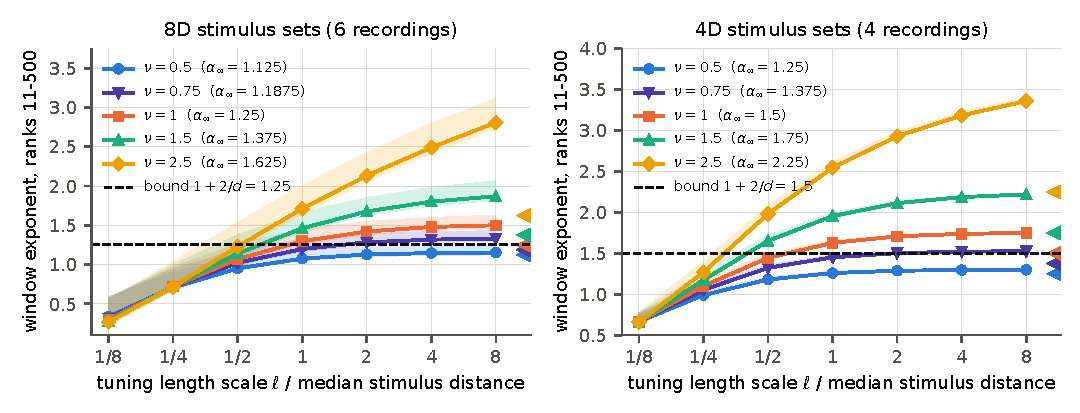
\includegraphics[width=0.94\textwidth]{figures/fig1.pdf}
\caption{Ranks 11--500 window exponent of noise-free Mat\'ern codes (infinitely many neurons) on the real stimulus coordinates, against the tuning length scale. Lines: median over the stimulus sets; bands: range over the sets. Arrowheads on the right: $\alpha_\infty = 1 + 2\nu/d$. Dashed line: the bound $1 + 2/d$. Deterministic. Table~\ref{tab:sens} gives the effect of finite populations, the rank window, the metric and the number of stimuli.}\label{fig:window}
\end{figure}

\begin{table}[t]
\centering\footnotesize
\caption{Ranks 11--500 window exponent of noise-free Mat\'ern codes (infinitely many neurons) on the real stimulus coordinates: range over the six 8D and the four 4D stimulus sets. Deterministic; no sampling error.}\label{tab:window}
\setlength{\tabcolsep}{3.5pt}
\begin{tabular}{ccc*{7}{c}}
\toprule
& & & \multicolumn{7}{c}{length scale $\ell$ / median pairwise distance} \\
\cmidrule(lr){4-10}
$d$ & $\nu$ & $\alpha_\infty$ & 1/8 & 1/4 & 1/2 & 1 & 2 & 4 & 8 \\
\midrule
8 & 0.5 & 1.125 & 0.30--0.59 & 0.67--0.90 & 0.93--1.09 & 1.05--1.18 & 1.10--1.22 & 1.12--1.23 & 1.12--1.24 \\
8 & 0.75 & 1.1875 & 0.27--0.58 & 0.68--0.94 & 0.99--1.19 & 1.17--1.33 & 1.25--1.39 & 1.28--1.42 & 1.29--1.43 \\
8 & 1 & 1.25 & 0.26--0.57 & 0.68--0.97 & 1.04--1.26 & 1.26--1.45 & 1.38--1.55 & 1.44--1.60 & 1.46--1.63 \\
8 & 1.5 & 1.375 & 0.23--0.56 & 0.67--1.00 & 1.10--1.38 & 1.41--1.67 & 1.62--1.85 & 1.75--1.98 & 1.82--2.07 \\
8 & 2.5 & 1.625 & 0.21--0.55 & 0.67--1.04 & 1.18--1.54 & 1.64--2.01 & 2.05--2.42 & 2.41--2.80 & 2.73--3.11 \\
\addlinespace
4 & 0.5 & 1.25 & 0.64--0.76 & 0.97--1.04 & 1.17--1.21 & 1.25--1.28 & 1.28--1.30 & 1.29--1.31 & 1.30--1.31 \\
4 & 0.75 & 1.375 & 0.63--0.77 & 1.03--1.12 & 1.31--1.36 & 1.45--1.48 & 1.50--1.52 & 1.52--1.53 & 1.52--1.54 \\
4 & 1 & 1.5 & 0.62--0.77 & 1.08--1.18 & 1.43--1.49 & 1.62--1.66 & 1.70--1.73 & 1.73--1.75 & 1.75--1.76 \\
4 & 1.5 & 1.75 & 0.62--0.77 & 1.14--1.28 & 1.63--1.72 & 1.95--2.00 & 2.11--2.14 & 2.18--2.21 & 2.21--2.23 \\
4 & 2.5 & 2.25 & 0.61--0.78 & 1.23--1.40 & 1.96--2.09 & 2.53--2.62 & 2.91--2.98 & 3.17--3.23 & 3.34--3.40 \\
\bottomrule

\end{tabular}
\end{table}

With infinitely many neurons the border codes ($\nu = 1$) give window exponents from \WinBorderEightMin{} to \WinBorderEightMax{} at $d = 8$ (bound 1.25) and from \WinBorderFourMin{} to \WinBorderFourMax{} at $d = 4$ (bound 1.50) (Figure~\ref{fig:window}, Table~\ref{tab:window}). They lie below the bound in every stimulus set for $\ell \le \CrossBelowEight$ at $d = 8$ and $\ell \le \CrossBelowFour$ at $d = 4$, and above it in every set for $\ell \ge \CrossAboveEight$ at $d = 8$ and $\ell \ge \CrossAboveFour$ at $d = 4$. The smoothness of these codes is fixed; the length scale moves the exponent across the bound, as Example~3 of \cite{stringer2019} anticipates for a single tuning radius. The stimulus set matters as well: at $\ell = 1$ the border code gives \WinBorderEightLOneMin{} to \WinBorderEightLOneMax{} across the 8D sets, the larger values in the sets with the smaller participation ratios, and \WinBorderFourLOneMin{} to \WinBorderFourLOneMax{} across the 4D sets. Differentiable codes fall below the bound at short length scales: at $\ell = 1/4$ the largest exponent over the 8D sets is \WinSmoothEightLQuarterMax{} for $\nu = 1.5$ and \WinSmootherEightLQuarterMax{} for $\nu = 2.5$, and over the 4D sets \WinSmoothFourLQuarterMax{} and \WinSmootherFourLQuarterMax{}. At long length scales they overshoot their own asymptotic exponent ($\nu = 2.5$ at $d = 4$ reaches \WinSmootherFourMax{} against $\alpha_\infty = 2.25$). Codes of fixed smoothness also reproduce the ordinal pattern that Stringer et al.\ predicted: in all \OrdinalTotal{} combinations of $\nu$ and $\ell$, every 4D set gives a larger exponent than every 8D set.

\subsection{How far these statements carry}

\begin{table}[t]
\centering\footnotesize
\caption{Ranks 11--500 window exponent of the border codes ($\nu = 1$) and of codes below the border ($\nu = 0.75$) under changes of the computation: range over the stimulus sets, with the number of sets above the bound $1 + 2/d$ in parentheses. $N = \infty$: Table~\ref{tab:window}. $N = 8{,}704$: mean over finite populations. 101--500: the same spectra fitted over ranks 101--500. Whitened: coordinates scaled to unit variance. $P$: mean over 4 random subsets of the stimuli.}\label{tab:sens}
\setlength{\tabcolsep}{3pt}
\begin{tabular}{ccc*{6}{c}}
\toprule
$d$ & $\nu$ & $\ell$ & $N = \infty$ & $N = 8{,}704$ & ranks 101--500 & whitened & $P = 1{,}400$ & $P = 2{,}000$ \\
\midrule
8 & 1 & 1 & 1.26--1.45 (6) & 1.24--1.44 (5) & 1.19--1.35 (2) & 1.13--1.19 (0) & 1.20--1.41 (2) & 1.24--1.43 (4) \\
8 & 1 & 4 & 1.44--1.60 (6) & 1.42--1.59 (6) & 1.30--1.43 (6) & 1.30--1.36 (6) & 1.38--1.56 (6) & 1.41--1.58 (6) \\
8 & 1 & 8 & 1.46--1.63 (6) & 1.44--1.62 (6) & 1.31--1.44 (6) & 1.33--1.38 (6) & 1.41--1.59 (6) & 1.44--1.61 (6) \\
8 & 0.75 & 4 & 1.28--1.42 (6) & 1.26--1.40 (6) & 1.13--1.24 (0) & 1.17--1.21 (0) & 1.21--1.36 (3) & 1.25--1.39 (6) \\
8 & 0.75 & 8 & 1.29--1.43 (6) & 1.27--1.41 (6) & 1.13--1.25 (0) & 1.18--1.23 (0) & 1.22--1.37 (4) & 1.26--1.40 (6) \\
\addlinespace
4 & 1 & 1 & 1.62--1.66 (4) & 1.62--1.66 (4) & 1.62--1.64 (4) & 1.60--1.63 (4) & 1.60--1.65 (4) & 1.61--1.65 (4) \\
4 & 1 & 4 & 1.73--1.75 (4) & 1.73--1.75 (4) & 1.66--1.67 (4) & 1.74--1.75 (4) & 1.72--1.74 (4) & 1.73--1.75 (4) \\
4 & 1 & 8 & 1.75--1.76 (4) & 1.74--1.76 (4) & 1.66--1.67 (4) & 1.76--1.76 (4) & 1.73--1.75 (4) & 1.74--1.76 (4) \\
4 & 0.75 & 4 & 1.52--1.53 (4) & 1.51--1.53 (4) & 1.43--1.44 (0) & 1.53--1.53 (4) & 1.48--1.50 (1) & 1.50--1.52 (4) \\
4 & 0.75 & 8 & 1.52--1.54 (4) & 1.51--1.53 (4) & 1.43--1.44 (0) & 1.53--1.54 (4) & 1.49--1.51 (1) & 1.51--1.52 (4) \\
\bottomrule

\end{tabular}
\end{table}

Table~\ref{tab:sens} tests these statements against the choices behind them. With 8,704 neurons the window exponents are mostly lower: over the \FinCells{} computed cells the mean shift ranges from \FinShiftMin{} to \FinShiftMax{}, and the \FinHigherN{} cells that rise are codes with $\nu = 1.5$ or $2.5$; between populations the standard deviation is only \FinSDMin{} to \FinSDMax{}. The border codes then lie below the bound in every set for $\ell \le \FinCrossBelowEight$ at $d = 8$ and $\ell \le \FinCrossBelowFour$ at $d = 4$, and above it in every set for $\ell \ge \FinCrossAboveEight$ at $d = 8$ and $\ell \ge \FinCrossAboveFour$ at $d = 4$ ($\ell = 1/8$ was not computed at finite $N$); at $\ell = 1$ they give \FinOneEightMin{} to \FinOneEightMax{} across the 8D sets, with \FinOneNearEight{} within 0.005 of the bound or below it. In the unwhitened coordinates they reach the reported exponents, 1.49 at $d = 8$ and 1.65 at $d = 4$, in \FinReachEight{} of the six 8D sets and in \FinReachAllFour{} four 4D sets, over the length scales computed (up to $\ell = 8$). The 8D count rests on a small margin: \FinReachMarginSetEight{} reaches \FinReachMarginEight{} above 1.49, with a standard deviation of \FinReachMarginSDEight{} over its \FinReachMarginREight{} populations. In whitened coordinates no 8D border code reaches 1.49: the largest value, with infinitely many neurons, is \WhiteBorderEightMaxAll{}, at $\ell = \WhiteBorderEightMaxAllEll$, the longest length scale computed. The 4D sets still reach 1.65 there (\WhiteBorderFourLEightMin{} to \WhiteBorderFourLEightMax{} at $\ell = 8$). For non-identification an existence statement in one metric suffices, but the 8D count holds only in the unwhitened metric.

For $\nu = 0.75$ the expected squared gradient diverges and $\alpha_\infty = 1 + 1.5/d$ lies below the bound (1.1875 at $d = 8$, 1.375 at $d = 4$). Over ranks 11--500, in the unwhitened coordinates and at 2,800 stimuli, these codes nevertheless exceed the bound at $\ell = 4$ in every set, with infinitely many neurons (\WinMidEightLFourMin{} to \WinMidEightLFourMax{} at $d = 8$, \WinMidFourLFourMin{} to \WinMidFourLFourMax{} at $d = 4$) and with 8,704 neurons in \FinMidAbovePhraseEight{} and \FinMidAbovePhraseFour{}. This is an existence statement for that window, that metric and that number of stimuli, and each matters. Over ranks 101--500 all \SubMidAboveCount{} cells of $\nu = 0.75$ that lie above the bound over ranks 11--500 fall below it (at $\ell = 4$: \SubMidEightLFourMin{} to \SubMidEightLFourMax{} at $d = 8$, \SubMidFourLFourMin{} to \SubMidFourLFourMax{} at $d = 4$). The spectra are curved: for $\ell \ge 1$ at $d = 8$ the ranks 11--100 exponent exceeds the ranks 101--500 exponent by a median of \CurvMedEight{} (over all cells the difference ranges from \CurvMin{} to \CurvMax{}), and for the \CurvBorderReachN{} border-code spectra that reach 1.49 in the 8D sets by \CurvBorderReachMin{} to \CurvBorderReachMax{}. We did not compute sub-window exponents of the recorded spectra, so whether spectra of this shape could stand in for the recorded ones is not tested here; the argument needs only that they give the same ranks 11--500 exponent. In whitened coordinates the $\nu = 0.75$ codes at $\ell = 4$ give \WhiteMidEightLFourMin{} to \WhiteMidEightLFourMax{} at $d = 8$, above the bound in \WhiteMidAboveEightWord{} of the six sets, while the 4D sets hardly change (\WhiteMidFourLFourMin{} to \WhiteMidFourLFourMax{}). The border codes keep landing on both sides in whitened coordinates: at $d = 8$ they give \WhiteBorderEightLOneMin{} to \WhiteBorderEightLOneMax{} at $\ell = 1$ and \WhiteBorderEightLEightMin{} to \WhiteBorderEightLEightMax{} at $\ell = 8$. With fewer stimuli the exponents fall: at $\ell = 4$ the 8D sets give \SubPOneThousandFourHundredMidEightLFourMin{} to \SubPOneThousandFourHundredMidEightLFourMax{} at $P = 1{,}400$ (above the bound in \SubPOneThousandFourHundredMidAboveEight{} of six sets) and \SubPTwoThousandMidEightLFourMin{} to \SubPTwoThousandMidEightLFourMax{} at $P = 2{,}000$ (above the bound in \SubPTwoThousandMidAboveEight{}; in \SubPTwoThousandMarginSet{} by only \SubPTwoThousandMarginMin{}, with a standard deviation over subsets of \SubPTwoThousandMarginSD{} and one subset at \SubPTwoThousandMarginSubMin{}). The subsets sample the same operator, so at 2,800 stimuli the window exponent still depends on the number of stimuli; its limit as $P$ grows, the window exponent of the operator eigenvalues at ranks 11--500, cannot be computed from these stimulus sets. Solving $w = 1 + 2\nu/d_{\mathrm{eff}}$ for $d_{\mathrm{eff}}$ at $\ell = 8$ gives $\DeffEightMin$ to $\DeffEightMax$ in the 8D sets and $\DeffFourMin$ to $\DeffFourMax$ in the 4D sets for the border codes, and $\DeffMidEightMin$ to $\DeffMidEightMax$ and $\DeffMidFourMin$ to $\DeffMidFourMax$ for $\nu = 0.75$. Because the two differ, $d_{\mathrm{eff}}$ is a descriptive rescaling of the window exponent, not a property of the stimulus set. The nearest-neighbour dimension, which is a property of the stimuli, is also below the nominal $d$ (Section~\ref{sec:geometry}), and this is consistent with codes below the border exceeding the nominal bound.

\subsection{Gratings, \texorpdfstring{$d = 1$}{d = 1}}\label{sec:d1}

\begin{figure}[t]
\centering
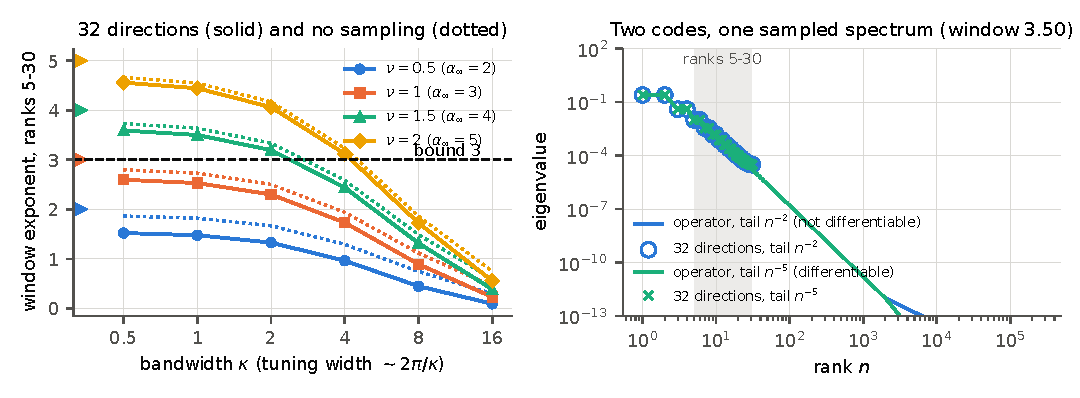
\includegraphics[width=0.94\textwidth]{figures/fig2.pdf}
\caption{Left: ranks 5--30 window exponent for 32 equally spaced directions (solid) and for the operator spectrum without sampling (dotted), against the bandwidth $\kappa$ of the tuning; arrowheads: $\alpha_\infty = 1 + 2\nu$; dashed: the bound 3. Right: the numerical example of Proposition~\ref{prop:window}. Two codes share the differentiable $\nu = 1.5$, $\kappa = 1$ spectrum up to frequency 1,000 and continue as $n^{-2}$ (not differentiable) or $n^{-5}$ (differentiable). Lines: operator spectra; markers: their 32-direction spectra, which coincide; both have window exponent \PropWSmoothA{}, above the bound 3.}\label{fig:d1}
\end{figure}

For every code of the family $c_k = (1 + k^2/\kappa^2)^{-(\nu + 1/2)}$ that we computed, the 32-direction window exponent lies below $\alpha_\infty$, by \GratShortMin{} to \GratShortMax{} (Figure~\ref{fig:d1}). The shortfall has two parts. The operator spectrum is itself shallower than $\alpha_\infty$ over ranks 5--30, by \GratPreMin{} to \GratPreMax{}, because it is flat for frequencies below $\kappa$ and because each frequency carries two equal eigenvalues; even an exact power law $c_k = k^{-3}$ gives \StairThree{} over ranks 5--30. Sampling at 32 directions folds the frequencies above 16 onto lower ones and lowers the exponent by a further \GratAliasMin{} to \GratAliasMax{} (aliasing). The border codes give \GratBorderMin{} to \GratBorderMax{}, all below 3, while differentiable codes with $\nu = 1.5$ give \GratNuOnePointFiveMin{} to \GratNuOnePointFiveMax{} and exceed 3 for $\kappa \le \GratSmoothAboveKappaMax{}$. Within this family and over the bandwidths computed, a 32-direction exponent above 3, such as 3.43, comes only from differentiable codes. Outside the family it does not. In the example of Figure~\ref{fig:d1}, two codes share the $\nu = 1.5$, $\kappa = 1$ spectrum up to frequency 1,000 and continue as $n^{-2}$ (not differentiable) or $n^{-5}$; their tail masses are \PropTailSmoothA{} and \PropTailSmoothB{}, their 32-direction eigenvalues differ by at most \PropRelSmooth{} of the 30th eigenvalue, and both have window exponent \PropWSmoothA{}, the value of the family code: a non-differentiable code gives a 32-direction exponent above the bound. Finite populations of 8,704 neurons changed the 32-direction exponent by at most \GratFinShiftMax{} on average, with a standard deviation of at most \GratFinSDMax{}.

\subsection{The broken-power-law tail exponent}

\begin{figure}[t]
\centering
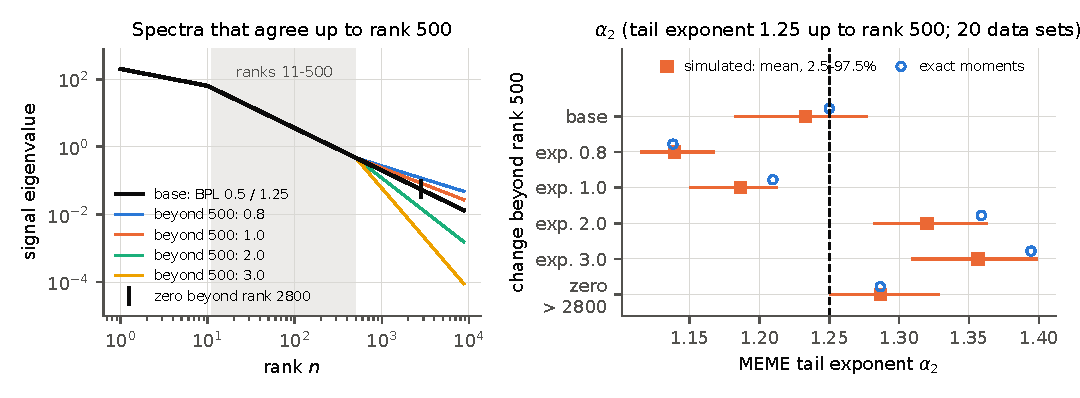
\includegraphics[width=0.94\textwidth]{figures/fig3.pdf}
\caption{Left: the base spectrum, a broken power law with exponents 0.5 and 1.25, and variants that agree with it up to rank 500; shaded: ranks 11--500. Right: MEME $\alpha_2$ (diagonal weights) for each spectrum; squares and bars, mean and 2.5th--97.5th percentiles over 20 simulated data sets with common random numbers; circles, the fit to the exact moments. Dashed: the base tail exponent 1.25.}\label{fig:meme}
\end{figure}

\begin{table}[t]
\centering\footnotesize
\caption{MEME broken-power-law tail exponent $\alpha_2$ for spectra that differ from the base broken power law beyond rank 500 (a different exponent, or zero after rank 2,800) or at every rank (a floor adding 5\% or 15\% of the base variance, or a factor $e^{-n/1000}$). Window: ranks 11--500 exponent of the true spectrum. Trace: variance relative to the base. Exact: fit to the exact moments, diagonal weights (diag.) and full whitening (full). Simulated (diagonal weights): mean $\pm$ standard error over 20 data sets, and the paired difference from the base with its 95\% interval. Flagged: fraction of the 20 data sets whose misfit exceeds the 95th percentile of the correctly specified model, diagonal and full. Last column: the same variants of a base with $\alpha_2 = 1.5$, exact moments, diagonal weights.}\label{tab:meme}
\setlength{\tabcolsep}{2.6pt}
\begin{tabular}{lccccccccc}
\toprule
& & & \multicolumn{6}{c}{base $\alpha_2 = 1.25$} & $\alpha_2 = 1.5$ \\
\cmidrule(lr){4-9}\cmidrule(lr){10-10}
& & & \multicolumn{2}{c}{exact} & \multicolumn{2}{c}{simulated} & \multicolumn{2}{c}{flagged} & exact \\
\cmidrule(lr){4-5}\cmidrule(lr){6-7}\cmidrule(lr){8-9}
change & window & trace & diag. & full & $\alpha_2$ & paired difference & diag. & full & \\
\midrule
none & 1.250 & 1.000 & 1.250 & 1.250 & 1.233 $\pm$ 0.006 &  & 0.05 & 0.00 & 1.500 \\
exponent 0.8 after 500 & 1.250 & 1.142 & 1.138 & 1.144 & 1.139 $\pm$ 0.004 & $-0.094$ [$-0.103$, $-0.085$] & 0.00 & 0.00 & 1.405 \\
exponent 1.0 after 500 & 1.250 & 1.064 & 1.210 & 1.207 & 1.187 $\pm$ 0.004 & $-0.047$ [$-0.054$, $-0.039$] & 0.00 & 0.00 & 1.442 \\
exponent 2.0 after 500 & 1.250 & 0.914 & 1.359 & 1.350 & 1.320 $\pm$ 0.006 & $+0.087$ [$+0.077$, $+0.097$] & 0.00 & 0.00 & 1.529 \\
exponent 3.0 after 500 & 1.250 & 0.879 & 1.394 & 1.386 & 1.357 $\pm$ 0.007 & $+0.123$ [$+0.113$, $+0.134$] & 0.00 & 0.00 & 1.552 \\
zero after 2,800 & 1.250 & 0.950 & 1.286 & 1.289 & 1.287 $\pm$ 0.006 & $+0.053$ [$+0.044$, $+0.063$] & 0.00 & 0.00 & 1.518 \\
\addlinespace
floor 5\% & 1.243 & 1.050 & 1.218 & 1.216 &  & & &  & 1.447 \\
floor 15\% & 1.230 & 1.150 & 1.135 & 1.141 &  & & &  & 1.311 \\
factor $e^{-n/1000}$ & 1.353 & 0.832 & 1.438 & 1.429 &  & & &  & 1.594 \\
\bottomrule

\end{tabular}
\end{table}

The variants in Table~\ref{tab:meme} agree with the base spectrum, a broken power law with tail exponent 1.25, up to rank 500. Beyond it they decay with exponent 0.8, 1.0, 2.0 or 3.0, or stop. Their exact-moment tail exponents range from \MemeTailMinA{} to \MemeTailMaxA{} (from \MemeTailMinB{} to \MemeTailMaxB{} for the base with 1.5): $\alpha_2$ moves toward the true continuation, by at most \MemeTailShiftMax{}, and stays far from it. No window of ranks up to 500 sees these changes. The eigenmoments see them through the trace, which changes by the factor \MemeTraceMin{} to \MemeTraceMax{}; one data set registers this (the log trace has a standard deviation of \MemeSDTrace{}), so the variance in the tail is observed. The moments $p \ge 2$ change by at most \MemeTailZMaxA{} standard deviations. The trace fixes how much variance lies in the tail, not how it decays. With diagonal weights the broken power law absorbs the change into $\alpha_2$: the exact-moment misfits are at most \MemeExactTailMisfitMax{}, against a null median of \MemeNullMedDiag{} and 95th percentile of \MemeNullQDiag{} over \MemeNB{} simulated data sets of the correctly specified model, and no data set of any variant is flagged (of the base, \MemeFlagDiagBaseN{} of 20); the median misfits of the variants, \MemeDiagVarMedMin{} to \MemeDiagVarMedMax{}, are even below that of the base, \MemeDiagBaseMed{}. With full-covariance whitening, closer to the check that Pospisil and Pillow propose (Section~1), the misfit of the correctly specified model has a heavy upper tail: median \MemeNullMedFull{} and 95th percentile \MemeNullQFull{} over the \MemeNB{} base data sets, against \ChiFourMed{} and \ChiFourQ{} for a chi-square distribution with 4 degrees of freedom (eight moments, four fitted parameters counting the profiled break). The five folds have medians \MemeFullFoldMeds{}; the last contributes \MemeFullNullExceedLast{} of the \MemeFullNullExceedAll{} misfits above the pooled 95th percentile, and the largest misfit is \MemeFullNullMax{}. The far-tail variants raise the median misfit of the simulated data sets from \MemeFullBaseMed{} to at most \MemeFullVarMedMax{}. How many of their data sets are flagged depends on the reference: none against the pooled 95th percentile, \MemeFlagFFMin{} to \MemeFlagFFMax{} against the 95th percentile of the first four folds (\MemeFullQFirstFour{}), \MemeFlagFOMin{} to \MemeFlagFOMax{} against that of the first fold, the 20 paired base data sets (\MemeFullQFirst{}), and \MemeLooFlagMin{} to \MemeLooFlagMax{} with the covariance estimated from only 19 data sets (the other paired sets, leaving one out), the exponent-0.8 variant most often. The misfit therefore has little power against these far-tail changes: nominal flag rates run from 0 to \MemeFlagAnyMax{}, depending on the reference distribution and the covariance estimate. The whitened fits shift $\alpha_2$ by similar amounts (exact moments: \MemeFullShiftThree{} for exponent 3.0, \MemeFullShiftPointEight{} for 0.8).

In the simulated data (Figure~\ref{fig:meme}) $\alpha_2$ of the base is \MemeSimBase{} $\pm$ \MemeSimBaseSE{}, with a standard deviation over data sets of \MemeSimBaseSD{}. The far-tail variants shift it by \MemeSimDiffMin{} to \MemeSimDiffMax{} (paired differences). The largest shift, \MemeSimDiffThree{} [\MemeSimDiffThreeLo{}, \MemeSimDiffThreeHi{}] for exponent 3.0, is \MemeRatioThreeSD{} times that standard deviation and \MemeRatioThreeGap{} of the gap of 0.20 between Pospisil and Pillow's average $\alpha_2$ of 1.20 and the natural-image bound of 1; for exponent 0.8 the shift is \MemeSimDiffPointEight{} [\MemeSimDiffPointEightLo{}, \MemeSimDiffPointEightHi{}]. Common random numbers helped only moderately: across data sets the $\alpha_2$ of a variant correlates with that of the base at \MemeCorrMin{} to \MemeCorrMax{}, and the paired differences have standard deviations of \MemePairedSDMin{} to \MemePairedSDMax{} against \MemeSimSDMin{} to \MemeSimSDMax{} for $\alpha_2$ itself. Changes that also touch ranks below 500 can move $\alpha_2$ further: a floor adding 15\% of the base variance lowers the window exponent only to \MemeFloorWinA{} but gives $\alpha_2 = \MemeFloorA{}$ (\MemeFloorB{} around 1.5).

For the Mat\'ern codes of Section~\ref{sec:theory} the relevant input is the set of eigenmoment estimates MEME would compute from their noise-free responses at the 2,800 stimuli (Section~\ref{sec:methods}); these estimate the population moments, not those of the 2,800-stimulus sample spectrum. The weights and the misfit threshold come from the simulated broken power law with neural noise, so for these noise-free moments the misfit is a heuristic filter, not a calibrated test. Many of these spectra are not broken power laws, and the diagonal-weight misfit shows it: its median over the \MemeMaternN{} codes computed is \MemeMaternMisfitMedian{}, far above the null. For $\ell \ge 1$ the profiled break sits at the lower edge of its grid, rank 4, in \MemeBrkLowDiag{} of \MemeBrkLowTotalDiag{} fits with either weighting, and at $\ell = 1/4$ it sits at the upper edge, rank 30, in \MemeBrkHighDiag{} diagonal-weight fits and \MemeBrkHighFull{} full-whitening fit; one diagonal-weight fit ends at the upper limit $\alpha_2 = 6$. These $\alpha_2$ are single-exponent fits from rank 4 onward rather than tail exponents in the usual sense. Among the \MemeGoodN{} fits whose diagonal-weight misfit lies within the null 95th percentile, \MemeGoodSmoothBelow{} of the \MemeGoodSmoothN{} differentiable codes ($\nu = 1.5$) have $\alpha_2$ below the bound and \MemeGoodRoughAbove{} of the \MemeGoodRoughN{} codes with $\nu = 0.75$ have $\alpha_2$ above it, and the border codes fall below it in \MemeGoodBorderBelow{} and above it in \MemeGoodBorderAbove{} cases. The full-whitening misfit passes a different set of \MemeFullGoodN{} fits: \MemeFullGoodSmoothBelow{} of its \MemeFullGoodSmoothN{} differentiable codes lie below the bound, \MemeFullGoodRoughAbove{} of its \MemeFullGoodRoughN{} codes with $\nu = 0.75$ above it, and its border codes \MemeFullGoodBorderBelow{} below and \MemeFullGoodBorderAbove{} above. Under either check, the tail exponents of passing fits lie on both sides of the bound for every smoothness computed. These moments are for infinitely many neurons, while the fit runs over 8,704 indices; for a population of $N$ Gaussian-process neurons $\mathbb{E}\operatorname{tr}\Sigma^2$ exceeds the infinite-population value by a relative amount of about $\mathrm{PR}/N$, with $\mathrm{PR} = (\operatorname{tr}\Sigma)^2/\operatorname{tr}\Sigma^2$ the participation ratio. PR reaches \MemePRMaxQuarter{} at $\ell = 1/4$ in the 8D sets and is at most \MemePRMaxOne{} for $\ell \ge 1$ (a relative change of at most \MemePRRelMaxOne\%). With the moments of a population of 8,704 neurons at $\ell = 1/4$, $\log\operatorname{tr}\Sigma^2$ rises by up to \MemeNLogTwoMax{} (\MemeNLogTwoSD{} weight standard deviations) and $\alpha_2$ changes by at most \MemeNAlphaShiftMax{}; every one of these fits stays below the bound, the number that pass rises from \MemeNPassInfDiag{} to \MemeNPassFinDiag{} of 30 with diagonal weights and from \MemeNPassInfFull{} to \MemeNPassFinFull{} with full whitening, and the statement about both sides of the bound still holds. These fits cover a restricted grid ($\nu \in \{0.75, 1, 1.5\}$, $\ell \in \{1/4, 1, 4\}$).

\subsection{cvPCA bias and the noise level}

The simulations of the preceding analysis found large downward biases of the cvPCA window exponent in conditions whose simulated cvPCA spectra lay far below the calibration recording's in the tail. In the repeated computation (broken power law, $\alpha_2 = 1.5$, realized window slope \SnrTruth{}) the bias was \SnrBiasOne{} $\pm$ \SnrSEOne{} with the calibrated noise, \SnrBiasFour{} $\pm$ \SnrSEFour{} with the non-aligned noise divided by 4, and \SnrBiasSixteen{} $\pm$ \SnrSESixteen{} with it divided by 16. None of the three conditions matches the recording: its cvPCA spectrum at ranks 11, 100 and 500 was (\SnrRatioOne{}), (\SnrRatioFour{}) and (\SnrRatioSixteen{}) times the simulated one in the three conditions, so in every condition the simulated cvPCA spectrum lies below the recording's at these ranks. The bias shrinks in magnitude as the noise is reduced, but we computed no signal-to-noise ratio of the tail, for the simulations or for any recording, so these biases cannot be transferred to the data. It does not bear on identifiability, which concerns the noise-free spectrum.


\section{Discussion}\label{sec:discussion}

\paragraph{What the reported exponents can show.} The exponents 1.49, 1.65 and 3.43 of \cite{stringer2019} are descriptive statistics of particular stimulus sets over particular rank windows. They are consistent with the bound, since codes that satisfy it can produce them. They cannot show that the code satisfies it, nor the stronger conclusions that it is ``as high-dimensional as possible'' or that the asymptotic exponent is close to $1 + 2/d$ (the fitted exponents are ``near but above the lower bounds''; the objection is to reading them as the asymptotic exponent), because codes that violate the bound, or sit exactly at it, produce the same window exponents. Border codes with 8,704 neurons reach 1.49 in \FinReachEight{} of the six 8D sets in the unwhitened coordinates (in whitened ones none does with infinitely many neurons) and 1.65 in \FinReachAllFour{} four 4D sets; codes below the border exceed the bound in some settings (Section~\ref{sec:results}); and on the torus a differentiable and a non-differentiable code can have finite-sample spectra that differ by less than any given amount at every rank, for every stimulus set (Corollary~\ref{cor:torus}). Conversely, a window exponent below $1 + 2/d$ would not show that a code is non-differentiable, since smooth codes with short length scales give such values. The ordinal prediction, larger exponents for lower $d$, is reproduced by codes of fixed smoothness, so its confirmation does not bear on smoothness either. A window exponent measures how the code's variance is spread over the modes the stimulus set resolves, at scales set by the tuning. This bears on the reanalysis of Davidovich and Roudi \cite{dr2022}, who found the 8D exponents above the bound ``with a reasonable margin'' and wrote that the uncertainty of the fits ``does not affect the conclusions regarding the smoothness of the population response to low-dimensional stimuli'': their result concerns the fitted exponent, and our computations say that even an exactly known window exponent does not decide smoothness. The broken-power-law tail exponent is likewise set by the assumed continuation beyond the resolved ranks: a tail that departs from the assumed form changes the trace, the fit absorbs this into $\alpha_2$, and the misfit has little power to detect it, with nominal flag rates from 0 to \MemeFlagAnyMax{} depending on the reference distribution and the covariance estimate. Pospisil and Pillow show that MEME recovers eigenvalues beyond the rank of the data when the parametric form is right (their Supplementary Fig.~S1, ``Demonstration that MEME estimator can infer eigenvalues beyond the rank of data''); they also note that the form of the tail ``remains unclear''.

\paragraph{What a test would need.} One route is many more stimuli per dimension, with the window moved to higher ranks as well: as $P$ grows, the fixed ranks 11--500 converge to the operator eigenvalues at those ranks, which for long tuning length scales remain pre-asymptotic, so more stimuli alone do not bring the window into the asymptotic regime. How many would be needed depends on the unknown length scale. A heuristic shows the scale of the problem: the nearest-neighbour spacing of $P$ stimuli in $d$ dimensions shrinks as $P^{-1/d}$, so resolving scales ten times shorter than 2,800 stimuli resolve now takes of the order of $10^d$ times as many stimuli. At $d = 1$ the obstacle is the number of directions: with 32 the window ends at the sampling frequency. The other route is a parametric model of the code, for example a kernel family such as \eqref{eq:matern} fitted to how response similarity falls with stimulus distance, with the bound read off the fitted smoothness. Such a test holds within the model, depends on the metric in which the code is assumed stationary, and meets the same resolution limit, because smoothness is decided at the shortest distances the stimulus set contains. Either route needs its assumptions stated in advance, and the geometry of each stimulus set, not only the nominal $d$, must enter the analysis.

\paragraph{Limitations.} The codes placed on the stimulus coordinates are isotropic, stationary Gaussian-process codes in the Euclidean metric of the image principal components, or of their whitened version. Real codes are neither isotropic nor stationary, and the metric in which the neural code is smooth is unknown; the family shows what the window exponent can do at fixed smoothness, not how visual cortex behaves. Proposition~\ref{prop:window} is proved for bounded eigenfunctions, and for the Mat\'ern codes on $\mathbb{R}^d$ we rely on computation. The identifiability computations are noise-free; estimation error comes on top. The MEME computations use one implementation with stated deviations from the authors' code, one noise model with fixed neurons and illustrative spectra, and for the Mat\'ern codes weights and a misfit threshold calibrated on a different spectrum; the size of the shifts in $\alpha_2$ depends on these choices, their existence does not. The stimulus-count dependence rests on 4 subsets per size. We make no statement about the exponents of the 8D, 4D or grating recordings. The bound of \cite{stringer2019} is a theorem, and nothing here questions it; the question is only whether data of this size can show that a code satisfies it.


\medskip
{\raggedright\noindent\textbf{Data and code availability.} The stimulus image files are part of the deposit of Stringer et al.\ on figshare, \url{https://doi.org/10.25378/janelia.6845348} (license CC BY-NC 4.0). The note's source folder lists the image files used, with their checksums, and holds the Python programs that produce every number, table and figure, their outputs and the commands to rerun them; it has not yet been deposited in a public archive.\par}

\noindent\textbf{Funding.} This research received no external funding.

\smallskip
\noindent{\footnotesize This work was prepared with AI assistance. The author takes full responsibility for its content.}

\begin{thebibliography}{10}
\footnotesize\raggedright

\bibitem{stringer2019} C. Stringer, M. Pachitariu, N. Steinmetz, M. Carandini and K. D. Harris, High-dimensional geometry of population responses in visual cortex, \emph{Nature} \textbf{571} (2019) 361--365; doi:10.1038/s41586-019-1346-5. Author manuscript PMC6642054; Supplementary Information read in part (Thms.~1, 2, 4, 5; \S\S2.1, 2.7, 3.5).

\bibitem{stringerdata} C. Stringer, M. Pachitariu, M. Carandini and K. Harris, Responses of ten thousand neurons to 2,800 natural images, figshare (2018); doi:10.25378/janelia.6845348.v3 (reference [36] of \cite{stringer2019}).

\bibitem{stringercode} MouseLand, \texttt{stringer-pachitariu-et-al-2018b}, \url{github.com/MouseLand/stringer-pachitariu-et-al-2018b}, commit 58443d1 (read: \texttt{python/utils.py}, \texttt{processResp/compileResps.m}).

\bibitem{pp2025} D. A. Pospisil and J. W. Pillow, Revisiting the high-dimensional geometry of population responses in the visual cortex, \emph{Proc. Natl. Acad. Sci. USA} \textbf{122} (2025) e2506535122; doi:10.1073/pnas.2506535122. Correction: e2533074122. SI Appendix read in part (captions of Figs.~S1, S2).

\bibitem{dr2022} I. A. Davidovich and Y. Roudi, Bayesian interpolation for power laws in neural data analysis, preprint, arXiv:2204.08525 (2022).

\bibitem{kg2000} V. Koltchinskii and E. Gin\'e, Random matrix approximation of spectra of integral operators, \emph{Bernoulli} \textbf{6} (2000) 113--167 (abstract read).

\bibitem{braun2006} M. L. Braun, Accurate error bounds for the eigenvalues of the kernel matrix, \emph{J. Mach. Learn. Res.} \textbf{7} (2006) 2303--2328.

\bibitem{stwck2005} J. Shawe-Taylor, C. K. I. Williams, N. Cristianini and J. Kandola, On the eigenspectrum of the Gram matrix and the generalization error of kernel-PCA, \emph{IEEE Trans. Inf. Theory} \textbf{51} (2005) 2510--2522 (read: Sects.~I--III).

\bibitem{kv2017} W. Kong and G. Valiant, Spectrum estimation from samples, \emph{Ann. Statist.} \textbf{45} (2017) 2218--2247 (read: arXiv:1602.00061v5, Sects.~1 and~3, Algorithm~1).

\bibitem{sgw2020} S. Spigler, M. Geiger and M. Wyart, Asymptotic learning curves of kernel methods: empirical data versus teacher--student paradigm, preprint, arXiv:1905.10843v8 (2020) (read: Sects.~1 and~7).

\bibitem{ppcode} D. A. Pospisil, \texttt{revisit\_hid\_geom}, \url{github.com/dapospisil/revisit_hid_geom}, commit afcd301 (read: \texttt{src/eig\_mom.py}).

\end{thebibliography}

\end{document}
